As indicated by Michael et al \cite{Michael2010ra}, an accurate simulation of a quadrotor is a valuable asset, which allows safe and efficient development of control algorithms. Additionally, it gives direct access to ground truth values and allows to design repeatable experiments.

This chapter proceeds as follows.
First, the AR.Drone simulation model is presented.
This simulation model consists of a motion model, visual model and sensor model.
In order to validate the methods presented in Section \ref{chapter:visual-slam} on both the real and the simulated AR.Drone, an abstraction layer is required.
This abstraction layer is part of the framework proposed in Section \ref{sec:proposed-framework}.

	\section{Simulation model}
The simulation environment selected is USARSim \cite{Balakirsky2009iros,carpin2007usarsim}, which is based on the Unreal Tournament game engine\footnote{\url{http://www.unrealengine.com}}.
It allows physical realistic simulations and includes a versatile environment editor.

		\subsection{USARSim simulation environment}
USARSim is an open source high fidelity robot simulator that can be used both for research and education.
It builds upon the Unreal Tournament game engine, a widely used and affordable state of the art commercial game engine.
The engine provides realistic rendering and physical simulation.
USARSim in itself is a set of models and a hierarchy of classes defining the simulation of robots, sensors and actuators.
The simulator is highly configurable and extendible: users can easily add new sensors or robots.
The level of effort devoted to validation has been a distinguishing feature of USARSim.
Each of its major constituents (e.g., robot kinematics, interaction with the environment, sensors, and camera video) have been subjected to ongoing validation testing \cite{formsma2011realistic,carpin2006high,wang2005validating,carpin2007bridging,carpin2006quantitative}.

USARSim was originally developed aiming to Urban Search And Rescue simulation.
The RoboCup Rescue league is part of the RoboCup\footnote{\url{http://www.robocup.org}} initiative.
This league aims at the development of robotics artifacts that could effectively help human rescuers in the aftermath of disasters like earthquakes, terroristic attacks, and other extreme situations.
In addition to a Rescue league with real robots, the Virtual Robots Competition was started, which uses USARSim as simulation environment.
%The first tournament took place during RoboCup 2006, with the participation of eight teams from four continents.

Another key feature of USARSim is the \textit{UnrealEd}\footnote{\url{http://nl.wikipedia.org/wiki/UnrealEd}} versatile environment editor.
The editor is part of Unreal Tournament and can be used to create an modify virtual environments.
It includes geometrical modeling tools which can import and export models compatible with most commercially available modeling software packages.
The details needed for an experiment or competition can be easily added (e.g., roads, fire).



		\subsection{Motion model}
The AR.Drone is a stabilized system (Figure \ref{fig:QuadRotorBody}). When no control signals are given the quadrotor hovers on the same location, which is accomplished by a feedback loop which uses the ultrasound sensor (for altitude) and the bottom camera (for horizontal position). The simulation makes use of this assumption. When no control signal is given, the AR.Drone stays at the same location.
When a control signal for a linear (forward/backward) or lateral (sideward) velocity is given, it calculates the force needed to reach that velocity (and assuming that the drag force $D_b$ increases linearly with the velocity). When the control signal stops, the drag force $D_b$ slows the quadrotor down until it hovers again.
The USARSim quadrotor model uses the Karma physics engine (part of the Unreal Engine \cite{Carpin2006}) to simulate the force and torque acting on the aircraft. Yet, only the overall thrust is calculated, the differential thrust is not used.
When moving in the horizontal plane, a real quadrotor changes its angle of attack (which is the defined as the angle between direction of motion $e_V$ and the body frame $e_N$ \cite{Yechout2003}). 
The Karma physics engine does not need this angle to calculate the resulting horizontal movement. Yet, this angle of attack has direct consequences for the viewing directions of the sensors, so the roll and the pitch should be adjusted in correspondence with horizontal movements. The active control of the AR.Drone is incorporated in the value of the dragforce $D_b$.

Control signals for vertical and rotational movements (around the z-axis) are calculated in the same manner. For vertical movements not only the drag force $D_b$ is taken into account. In this case also the gravitational force $mg$ is included in the equation. Rotations around the z-axis stop quite quickly when no control signal is given. For this rotational movement a strong drag force $D_r = 20 \times D_b$ is used to model the additional inertia. 

The principal elements of inertia are calculated correspondingly to $(0.0241, 0.0232, 0.0451)\small{kg\cdot m^2}$, assuming a homogeneous distribution of the mass.

The result is a simulation model which maneuvers in a way similar to the actual AR.Drone, as demonstrated in Section~\ref{sec:simulation_results}.


		\subsection{Sensor model}
The USARSim simulator has a set of configurable sensors, which include all the sensors from the AR.Drone.
Each mounted sensor is triggered at fixed time intervals (every $200\small{ms}$ by default).
The AR.Drone's time interval is reduced to $5\small{ms}$, producing up to 200 sensor measurements per second.

The ultrasound sensor emits a number of traces, which in combination form a cone.
First the sensor sends out one trace in the direction of its orientation remembering the measured range.
Then it does several conical measurements and calculates the minimal measured distance.
If the angle between a trace and the surface normal is smaller than angle $\alpha_{maxIncidence}$ the measurement is ignored.

\begin{figure}[htb!]
\centering
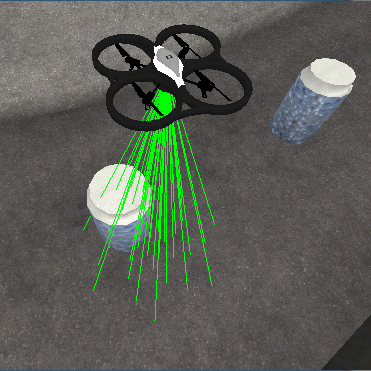
\includegraphics[width=6cm]{images/usarsim_sonar_beams.png}
\caption{The ultrasound sensor is modeled by emitting a number of traces, which in combination form a cone.} 
\label{fig:3Dmodel}
\end{figure}


The acceleration sensor computes the body accelerations using the AR.Drone's velocity:
\begin{equation}
a_{t} = (v_{t} - v_{t-\Delta t}) / \Delta t
\end{equation}
where $\Delta t$ is the time between measurements and $v$ is the velocity of the AR.Drone. The velocity of an object is modeled explicitly by the simulator.

The camera is modeled by creating a viewpoint in the Unreal engine.
%The sensors field of view property controls the camera's focal length.
The field of view is set to $64$ degrees and the resolution is set to $176 \times 144$ pixels, matching the specifications of the AR.Drone's bottom camera.
Camera calibration of the virtual camera was performed using OpenCV's Calibration tool\footnote{\url{http://opencv.willowgarage.com/documentation/camera_calibration_and_3d_reconstruction.html}}.
To do so, the calibration pattern was placed in a virtual enviroment and the AR.Drone manoeuvred above it.

\begin{figure}[htb!]
\centering
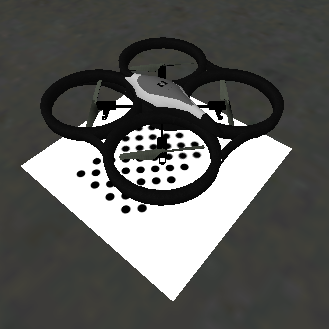
\includegraphics[width=6cm]{images/usarsim_camera_calibration.png}
\caption{Calibration of a virtual camera inside the USARSim simulator.} 
\label{fig:3Dmodel}
\end{figure}

USARSim supports dynamic lightning to produce realistic images and shadows.
However, the camera sensor lacks a noise model and doesn't emulate the effect of automatic white balancing that is performed in most cameras (including the AR.Drone's camera).
\cite{Visser2011imav} Briefly describes the influence of white balancing on image stitching and how to mimic the real images as close as possible.


		\subsection{Visual model}
In addition to the motion and sensor model, a visual model of the AR.Drone has been developed.
A highly detailed 3D model of the AR.Drone was provided by Parrot SA.
However, this model was unsuitable for simulation due to the computational complexity.
A simplified model (Figure~\ref{fig:3Dmodel}) was made using Blender\footnote{\url{http://www.blender.org/}}.
This model is optimized for simulation on consists of only 3142 vertices.
Both the simulated and real system have the same dimensions $(0.525,0.515,0.115)\small{m}$.
%The collision box (bounding box) was set

\begin{figure}[htb!]
\centering
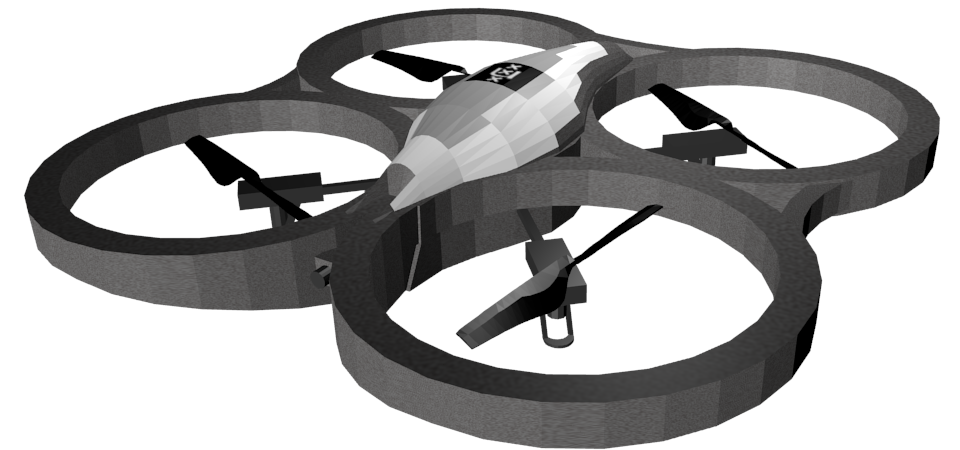
\includegraphics[width=6cm]{images/ardrone_blender_final.png}
\caption{3D model of the Parrot AR.Drone. This is a model optimized for simulation, based on the highly detailed model provided by Parrot SA.} 
\label{fig:3Dmodel}
\end{figure}


\section{Proposed framework}
\label{sec:proposed-framework}
The AR.Drone API (Section \ref{sec:API}) is the reference project for developing applications for the AR.Drone.
It provides basic functionality for communicating with the AR.Drone.
In order to perform advanced tasks (e.g., sensor data processing and automated drone control), a framework is proposed.
This framework includes an abstraction layer to abstract from the actual device.
Interfaces are used to connect the framework to an actual or virtual device.
Due to this abstraction, both the real and simulated AR.Drone can be used to validate the methods presented in the next chapter.

The main functionalities of the framework can be summarized as follows:
\begin{itemize}
\item Object-oriented programming: robots are represented with an object and are configured using parameters;
\item Abstraction from actual device: both the real and simulated AR.Drone can be connected to the framework;
\item Dataset recording and playback;
\item Queued sensor data and camera frame processing;
\item Keyboard controls;
\item Autonomous waypoint navigation;
\item Realtime 3D map visualization with freeflight
\end{itemize}

\begin{figure}[htb!]
\centering
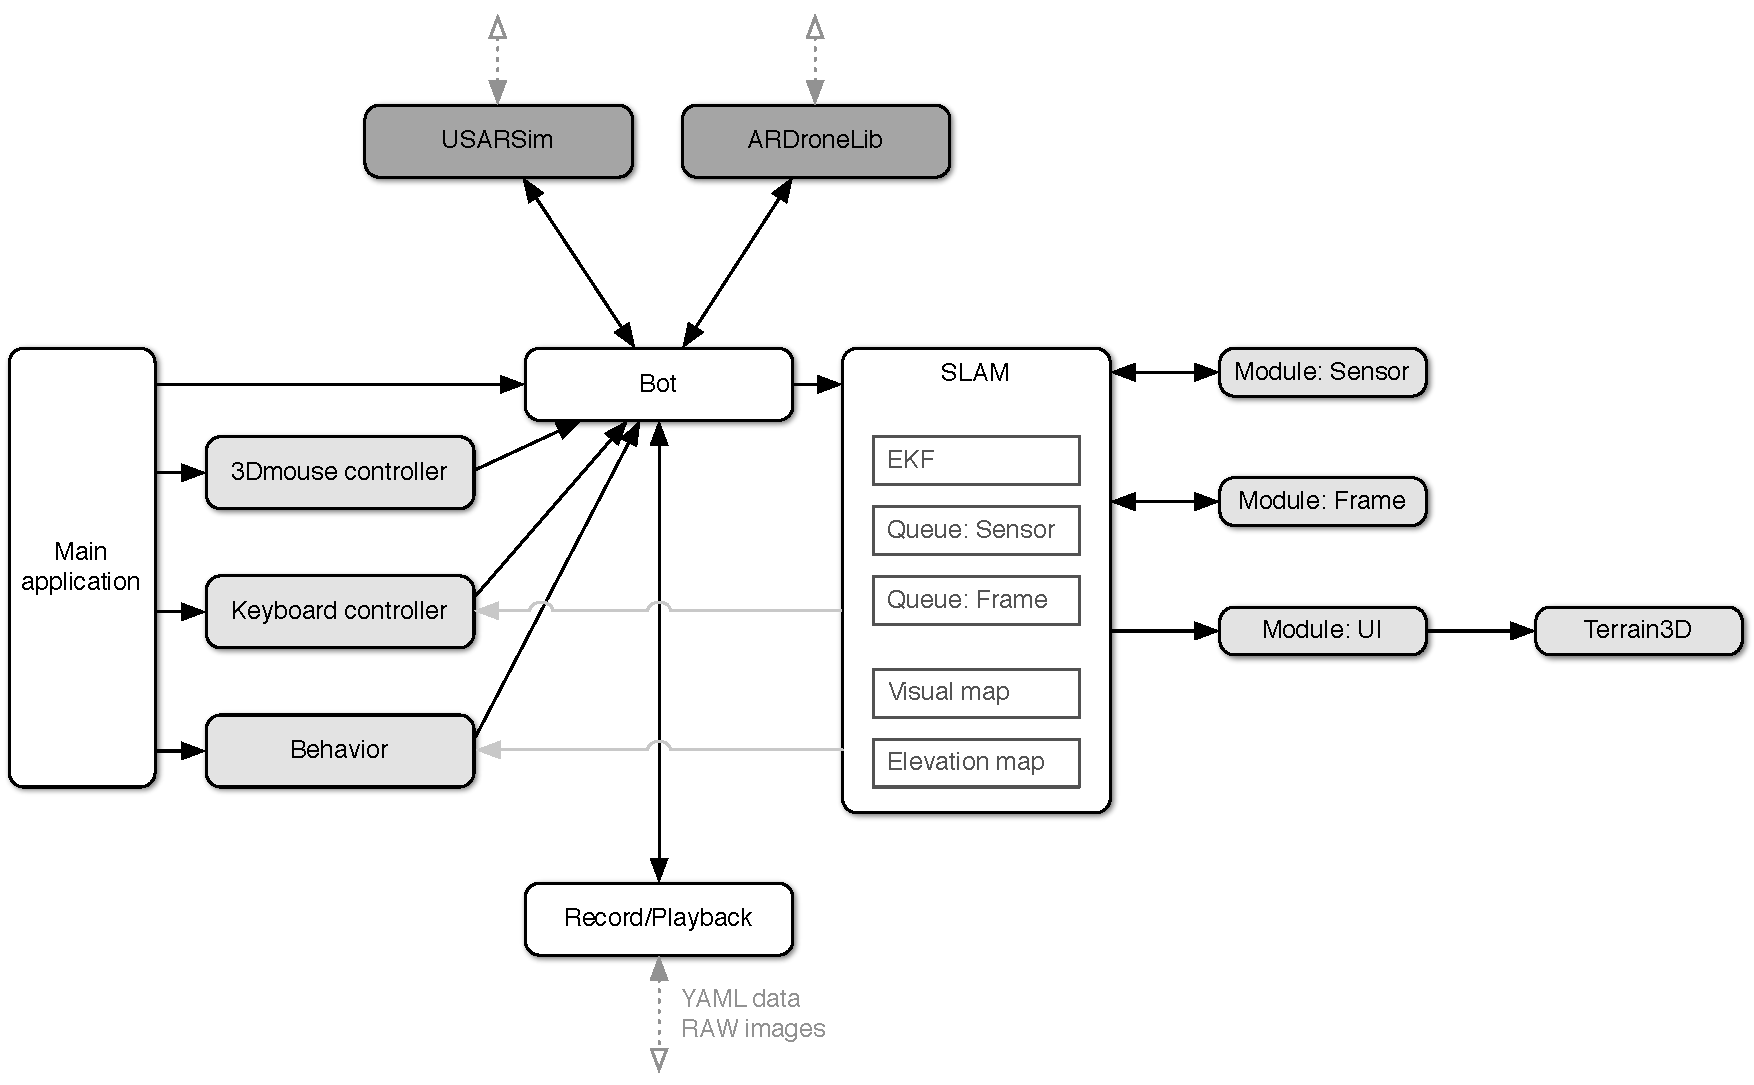
\includegraphics[width=\linewidth]{images/framework.pdf}
\caption{Schematic overview of the proposed framework. Each node respresents an object/datastructure. A light-gray node indicates the object is running in a dedicated thread. A dark-gray node indicates an interface to a device.} 
\label{fig:proposed_framework_schematic}
\end{figure}

A schematic overview of the framework is given in Figure \ref{fig:proposed_framework_schematic}.
The heart of the framework is the bot object, which respresents a robot.
Multiple robots can be instantiated simultaneous (e.g., a real and simulated AR.Drone).
The framework is limited to a single real AR.Drone's due to the lack of multirobot support in the ARDroneLib.
A robot is controlled by calling member functions of the corresponding bot instance.
Currently, three control methods are implemented: a \textit{keyboard controller}, a \textit{3D Mouse controller} and a \textit{behavior controller}.
Both the \textit{keyboard controller} and \textit{3D Mouse controller} can be used to manually fly the AR.Drone and manipulate the behavior of the SLAM system.
The \textit{behavior controller} is used to autonously fly the AR.Drone. 
It provides waypoint navigation to autonomously navigate the AR.Drone along a predefined route in world coordinates.
Feedback from the SLAM system (e.g., robot's estimated state) is used by the behavior controller to select the appropriate commands for the robot.

In addition to the controllers, a record and playback functionality is present.
Playback of a dataset is a valuable asset for testing.
All control commands sent to the drone and data received from the drone (i.e., navdata and camera frames) can be recorded to a dataset.
The data is stored in YAML\footnote{\url{http://en.wikipedia.org/wiki/YAML}} format.
When playing back a dataset, the data is pushed to the bot object in a way similar to regular data.
A timer is used to push the data at the appropriate timestamps, mimicing the original data as closely as possible.

An abstraction layer is used to abstract a bot from the actual device.
This enables to control both a real and simulated AR.Drone in the same manner.
\textit{Interfaces} are used to map a bot object to a (simulated) device.
When a bot object is instantiated, an interface has to be selected.
This can be either a real AR.Drone (using the ARDroneLib), simulated AR.Drone (USARSim) or use no interface for dataset playback (i.e., there is no communication with a robot).
The interface is responsible for transforming data received in device-specific format to a generic datastructure used by the framework.
Also, the control commands that are sent to the robot are transformed from generic format to device-specific format.

The data received from a robot (i.e., navdata and camera frames) is pushed to the SLAM object, which implements a SLAM system.
Navdata is added to the Sensor Queue, camera frames are added to the Frame Queue.
If the Frame Queue is not empty when a new frame is received (i.e., another frame is being processed), the frame is dropped by default.
The advantages of a queue are twofold: it allows data buffering and passing data to another thread to prevent blocking.
The latter is very important for a SLAM system, since blocking causes wasted data or delayed data.
The SLAM object has three modules: Sensor, Frame and UI.
Each module runs in a separate thread to prevent blocking and allow simultaneous data processing.
Both the Sensor and Frame module are able to update the EKF independently.

The \textbf{Sensor module} processes navdata (e.g., altitude and velocity estimates) from the AR.Drone at $200 \small{Hz}$.
When a navdata package is received, the EKF predicts a new state from the previous estimate (Section \ref{sec:background-solution-techniques}).
Each navdata package is processed before it can be used to update the estimated state of the AR.Drone.
This processing task includes the transformation of measurements to the global reference frame and the detection of obstacles.
The processed navdata is used to generate a measurement for the EKF.
Elements of the measurement matrix that cannot be (reliably) extracted from the processed navdata, are extraced from the prediced state and added to the measurement matrix with a higher covariance (uncertainty).
Finally, the measurement is used to update the state of the EKF.

The \textbf{Frame module} processes camera frames.
When a camera frame is received, the EKF predicts a new state from the previous estimate (Section \ref{sec:background-solution-techniques}).
Each camera frame is processed to extract information that is used to update the estimated state of the AR.Drone.
Processing includes Visual Odometry (Section \ref{sec:visual-slam-visual-odemetry}), updating the map (Section \ref{sec:mapping}) and recovering the global position of the AR.Drone by matching the frame against the map (Section \ref{sec:localization}).
The extracted information (i.e., velocities or global position) is used to generate a measurement for the EKF.
Elements of the measurement matrix that are be extracted from the camera frames (e.g., altitude), are extraced from the prediced state and added to the measurement matrix with a higher covariance (uncertainty).
Finally, the measurement is used to update the state of the EKF.

Processing a single frame may take up to $200 \small{ms}$ and causes a delay between input and updating the state.
This introduces a synchronization issue between state updates: when a update from the Frame module is applied, the estimated state is already updated by the Sensor module with more recent information that originates from the navdata.
This issue is solved by pausing the Sensor module (processing) while processing a frame.
After the state update by the Frame module is applied, the Sensor module is resumed and the queued navdata information is processed.

The \textbf{UI module} is responsible for visualizing the map.
It initializes a Terrain3D object and pushes local map updates to it.
The Terrain3D object renders the map (Figure \ref{fig:terrain3d_map}).
It allows 3D rendering of a textured elevation map.
Both the visual map and elevation map are integrated to a single map.
The code is based on the work by Chad Vernon \footnote{\url{http://www.chadvernon.com/blog/resources/directx9/moving-around-a-3d-world}} and uses DirectX 9 for rendering.
The estimated position of the AR.Drone is visualized with a red arrow.
\begin{figure}[htb!]
\centering
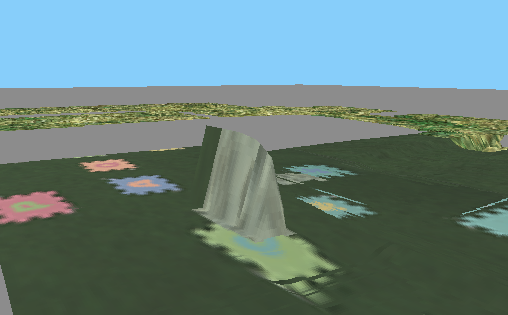
\includegraphics[width=6cm]{images/3dterrain_map.png}
\caption{Textured elevation map rendered by the Terrain3D object.} 
\label{fig:terrain3d_map}
\end{figure}